\documentclass[sigconf,nonacm]{acmart}

\usepackage{booktabs}

\settopmatter{printfolios=true}
% Lets TeX loosen a line instead of letting it run into the margin.
\setlength{\emergencystretch}{1.5em}

\begin{document}

\title{AutoDoomscroller: An On-Device Agent That Learns\\Which Short Videos You Would Skip}
\subtitle{Project Proposal}

\author{Juyong Park}
\affiliation{%
  \department{Business Administration}
  \institution{Seoul National University}
  \country{Republic of Korea}}
\email{tony3ynot@snu.ac.kr}

\begin{abstract}
Short-video feeds are ranked to keep people watching, yet in six days of our own logs 38\% of
the non-ad reels were swiped away within two seconds. We propose AutoDoomscroller, an Android agent
that learns from one person's scrolling which Instagram Reels and YouTube Shorts they would
skip, then skips them, lets them scroll and like with gestures, and shows them what they
watch. Everything runs on the phone. A prototype already records both apps, and a first model
reaches a skip AUC of 0.63.
\end{abstract}

\maketitle

\section{Motivation}
Scrolling a short-video feed means making the same small decision hundreds of times a day:
watch this, or swipe it away. In six days our prototype logged 1{,}833 reels. Of the non-ad
reels, 38\% were left within two seconds, half of those within about one second
(Fig.~\ref{fig:dwell}). The feed itself is chosen by the platform's recommender, which is
built to maximise watch time~\cite{covington2016youtube,zhan2022duration}, and users of such
feeds report a weakened sense of agency~\cite{lukoff2021youtube}.

We ask whether the phone can learn those quick judgements from the user's own behaviour and
act on them: skip what the user would skip anyway, let them move through the feed without
touching it, and show them where their time goes. Unlike the platform's recommender, such an
agent works for the user and keeps their data on the device. Building it touches every part of
a mobile ML system: sensing, on-device learning, model compression and visualization.

\begin{figure}[t]
  \centering
  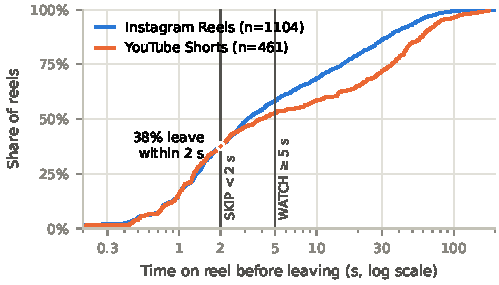
\includegraphics[width=\columnwidth]{figures/dwell_ecdf}
  \caption{Time spent on each non-ad reel before swiping away (six days, one user). In both
  apps 38\% of reels are left within 2\,s.}
  \label{fig:dwell}
\end{figure}

\section{Literature Review}
Platforms predict engagement from the logs of millions of users: YouTube ranks videos by
expected watch time~\cite{covington2016youtube}, Kuaishou corrects watch-time prediction for
video length~\cite{zhan2022duration}, and dwell time is a well-established signal of
preference~\cite{yi2014dwell}. EdgeRec even moves part of the ranking onto the phone so that it
reacts to the user's latest actions~\cite{gong2020edgerec}, but it still serves the platform's
goals. We instead predict one person's skips on their own phone, from a few hundred examples
and without access to the platform.

Digital self-control tools mostly block or limit use~\cite{lyngs2019selfcontrol}, and Lukoff
et al.\ found that autoplay and recommendations undermine users' sense of
agency~\cite{lukoff2021youtube}. Our agent does not block anything; it acts on the user's own
past choices and makes them visible.

For hands-free control, EyePhone showed early on that a phone can be operated with eye
blinks~\cite{miluzzo2010eyephone}, and MediaPipe now runs face and hand landmark models in real
time on phones~\cite{lugaresi2019mediapipe}. For the models we use MobileNetV3 on
frames~\cite{howard2019mobilenetv3} and multilingual E5 on text~\cite{wang2024me5}, and compress
them with integer quantization~\cite{jacob2018quantization} and pruning.

\begin{figure*}[t]
  \centering
  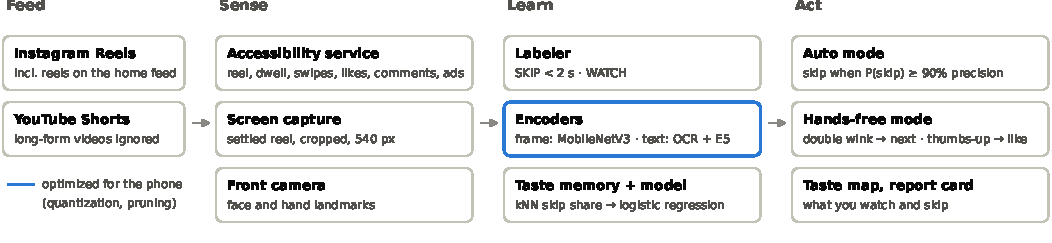
\includegraphics[width=\textwidth]{figures/overview}
  \caption{System overview. Everything runs on the phone.}
  \label{fig:overview}
\end{figure*}

\section{Proposed Design}
\textbf{Sense} (Fig.~\ref{fig:overview}). An accessibility service reads the screen of
Instagram Reels and YouTube Shorts a few times per second to know which reel is showing, how
long it stayed, and whether the user liked, saved or commented on it or watched it to the end.
Once a reel has settled after the swipe, the service takes one screenshot cropped to the reel.
In hands-free mode, the front camera is used for face and hand tracking.

\textbf{Label.} A reel counts as SKIP if the user left within 2\,s, and as WATCH if they
interacted with it, watched it to the end, or stayed at least 5\,s. Everything in between is
left out. Likes alone would not work as a target: there were only 6 in 1{,}833 reels.

\textbf{Learn.} The model may only use what is known when a reel appears: the first frame, the
text on it (read with on-device OCR such as ML Kit), the caption, and the creator's history.
For each of these we look up the most similar reels the user has already seen and use the share
of skips among them as a score; a logistic regression combines the scores into
$P(\text{skip})$. Because the scores come from a growing memory, the model keeps improving
without retraining the encoders.

\textbf{Act.} Auto mode swipes when $P(\text{skip})$ is high enough to be right 90\% of the
time; if the user goes back to an auto-skipped reel, that counts as a correction. Hands-free
mode maps a double wink to ``next'' and a thumbs-up to ``like''. A taste map and a per-session
report card show the user's habits.

\section{Prototype Implementation}
The Android app (Kotlin, tested on a Galaxy S24) already tracks both apps, detects and skips
ads, and exports its logs for offline analysis in Python, where we compute embeddings, run OCR
and evaluate models on days they were not trained on.

\begin{table}[t]
  \caption{Skip AUC on 933 labeled reels, each day predicted from the days before it (mean,
  95\% CI).}
  \label{tab:prelim}
  \small
  \begin{tabular}{@{}lc@{}}
    \toprule
    Inputs & Skip AUC \\
    \midrule
    Creator history & 0.63 (0.58--0.68) \\
    First frame (MobileNetV3) & 0.56 (0.52--0.61) \\
    Text on the frame (OCR) & 0.58 (0.53--0.62) \\
    Creator + frame + caption & 0.62 (0.57--0.67) \\
    \quad + session context & 0.56 (0.52--0.61) \\
    \bottomrule
  \end{tabular}
\end{table}

\textbf{Preliminary results.} Table~\ref{tab:prelim} shows the first results. The creator's
history alone reaches an AUC of 0.63; adding the frame and caption does not help yet. The most
promising content signal is the text on the frame: on reels where a sharper 540\,px frame is
available, its AUC rises from 0.46 to 0.63, so the app now captures that frame first.
Information about the session, such as time of day and recent scrolling pace, makes things
worse, because the user's mood changes from one session to the next.

\section{Potential Challenges}
\begin{itemize}
  \item \emph{Weak signal.} First impressions are noisy and depend on mood. Sharper on-screen
    text, per-session thresholds and online updates should help.
  \item \emph{Speed and battery.} Half of the quick skips happen within about a second, so
    capturing, reading and scoring a reel must take a few hundred milliseconds, and the
    screenshots and camera must not drain the battery.
  \item \emph{Measuring an agent that acts.} Auto-skipped reels lose their label, so a random
    10\% of predicted skips will be let through to measure precision.
  \item \emph{Fragility.} The app depends on the apps' screen layouts (partly on Korean UI
    text), and the data comes from one user.
  \item \emph{Privacy.} Screenshots and camera frames never leave the phone.
\end{itemize}

\section{Expected Outcomes and Plan}
(1)~An Android app with Learning, Auto and hands-free modes, with all inference on the phone.
(2)~A skip model with an AUC of at least 0.70 on unseen days and at least 90\% precision in
Auto mode. (3)~A compression study of the encoders (FP32, FP16, INT8 quantization, pruning)
reporting size, on-device latency and accuracy before and after. (4)~Battery use per mode, a
taste map and a report card.

\textbf{Plan.} Nov.~1--7: proposal; collect data with the new capture. Nov.~8--14: hands-free
mode. Nov.~15--21: better model; run it on the phone. Nov.~22--28: compression study; Auto
mode. Nov.~29--Dec.~5: measurements, visualization, final report.

\bibliographystyle{ACM-Reference-Format}
\bibliography{refs}

\end{document}
